\begin{flushleft}
{\large \textbf{介紹}}\\
\end{flushleft}

近年來硬體技術、軟體、自動求導等技術快速發展起來,再次帶起機器學習的發展,促使機器學習與各領域結合的應用越來越廣泛,在機電系統採用強化學習是為了讓機電系統的控制達到最佳化。本研究利用強化學習優化冰球機的對打系統,並測試相同演算法運用在2D與3D模擬環境可行性。\\

 本研究分成兩大部分,第一部分簡化冰球機並運用OpenAI Gym的Atari Pong-v0測試較合適的訓練參數,在2D環境中進行強化學習的對打訓練。第二部分獎實體系統簡化後導入CoppeliaSim模擬環境導入測試完成的訓練參數進行虛擬訓練,進行算法導入到實體機前的測試。\\

\begin{figure}[hbt!]
\begin{center}
\subfigure{
\begin{minipage}[t]{0.3\linewidth}  %設定圖片間距
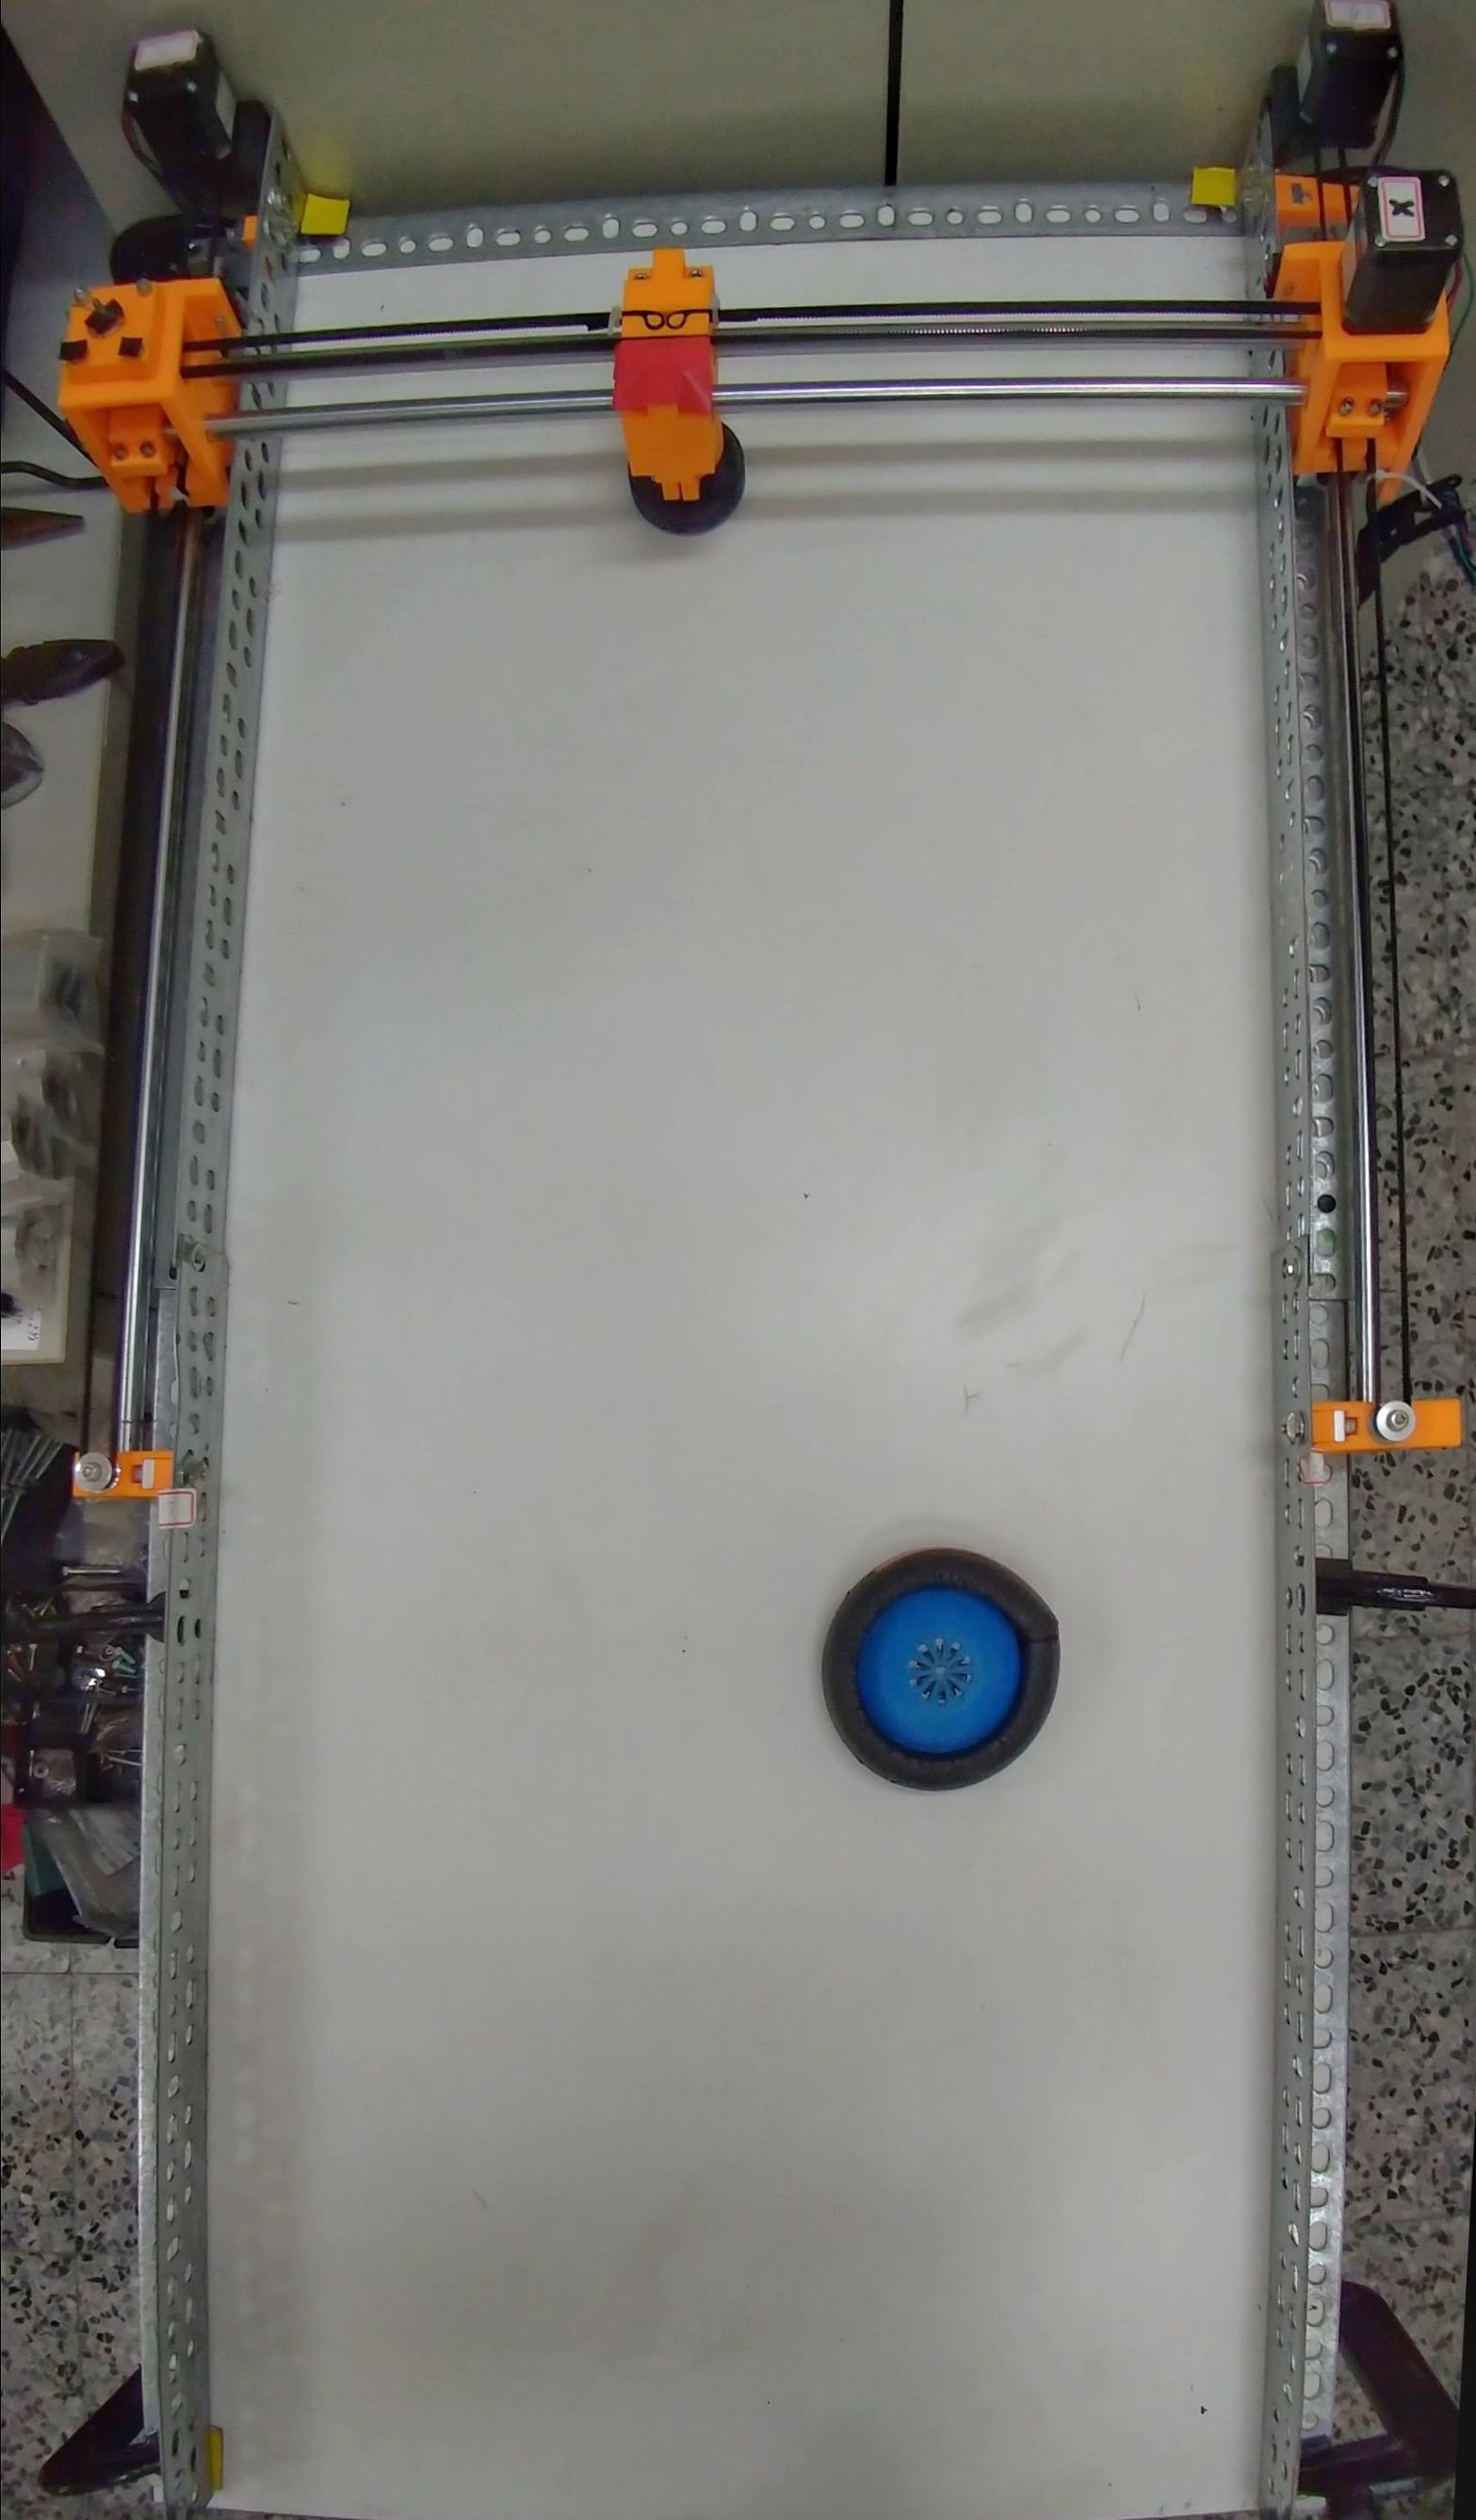
\includegraphics[width=4cm]{冰球機}
\caption{實體的冰球機}\label{fig.冰球機}
\end{minipage}
}
\subfigure{
\begin{minipage}[t]{0.3\linewidth}
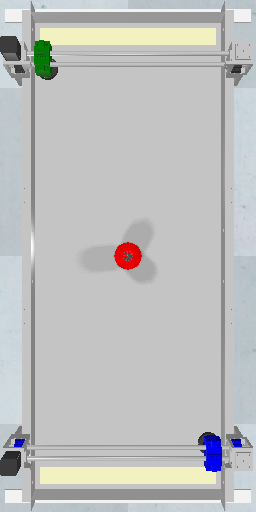
\includegraphics[width=4cm]{origin}
\caption{虛擬環境簡化後的冰球機}\label{fig.模擬冰球機}
\end{minipage}
}
\subfigure{
\begin{minipage}[t]{0.3\linewidth} 
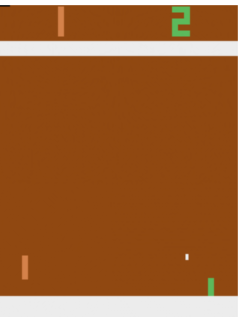
\includegraphics[width=4cm]{pong_gym}
\caption{Gym的Pong game}\label{fig.pong_gym}
\end{minipage}
}
\end{center}
\end{figure}
